% %% ----------------------------------------------------------------
%% Thesis.tex -- MAIN FILE (the one that you compile with LaTeX)
%% ---------------------------------------------------------------- 

% Set up the document
\documentclass[a4paper, 11pt, oneside]{Thesis}  % Use the "Thesis" style, based on the ECS Thesis style by Steve Gunn
\graphicspath{images/}  % Location of the graphics files 

% Include any extra LaTeX packages required
\usepackage[square, numbers, comma, sort&compress]{natbib}  % Use the "Natbib" style for the references in the Bibliography


\hypersetup{urlcolor=blue, colorlinks=true}  % Colours hyperlinks in blue, but this can be distracting if there are many links.

% new \oset macro:
\makeatletter
\newcommand{\oset}[3][0ex]{%
  \mathrel{\mathop{#3}\limits^{
    \vbox to#1{\kern-2\ex@
    \hbox{$\scriptstyle#2$}\vss}}}}
\makeatother

%% ----------------------------------------------------------------
\begin{document}
\frontmatter      % Begin Roman style (i, ii, iii, iv...) page numbering

\maketitle
%% ----------------------------------------------------------------

\setstretch{1.3}  % It is better to have smaller font and larger line spacing than the other way round

% Define the page headers using the FancyHdr package and set up for one-sided printing
\fancyhead{}  % Clears all page headers and footers
\rhead{\thepage}  % Sets the right side header to show the page number
\lhead{}  % Clears the left side page header

\pagestyle{fancy}  % Finally, use the "fancy" page style to implement the FancyHdr headers

%% ----------------------------------------------------------------

% The Abstract Page
\addtotoc{Abstract}  % Add the "Abstract" page entry to the Contents
\abstract{
\addtocontents{toc}{\vspace{1em}}  % Add a gap in the Contents, for aesthetics
blah\ldots

}

\clearpage  % Abstract ended, start a new page
%% ----------------------------------------------------------------

\setstretch{1.3}  % Reset the line-spacing to 1.3 for body text (if it has changed)

% The Acknowledgements page, for thanking everyone
\acknowledgements{
\addtocontents{toc}{\vspace{1em}}  % Add a gap in the Contents, for aesthetics

blah\ldots

}
\clearpage  % End of the Acknowledgements
%% ----------------------------------------------------------------

\pagestyle{fancy}  %The page style headers have been "empty" all this time, now use the "fancy" headers as defined before to bring them back


%% ----------------------------------------------------------------
\lhead{\emph{Contents}}  % Set the left side page header to "Contents"
\tableofcontents  % Write out the Table of Contents

%% ----------------------------------------------------------------

\mainmatter	  % Begin normal, numeric (1,2,3...) page numbering


% Include the chapters of the thesis, as separate files

\input{Chapters/01-kscont}
\chapter{CSW graph-theoretic approach to quantum correlations}
\lhead{\emph{CSW graph-theoretic approach to quantum correlations}}
\label{sec:csw}

In \cite{Cabello2014}, the authors propose a graph-theoretic approach to classifying the statistics of an arbitrary correlation experiment that aims to determine the value of some linear combination of probabilities. In particular, \cite{Cabello2014} identifies a hierarchical structure that classifies correlations as classical (KS non-contextual), quantum, or more generally obeying the exclusivity principle \footnote{The exclusivity applies to pairwise exclusive events and bars their added probabilities from exceeding 1. We will come back to it shortly.}. This hierarchical structure is established by associating with a correlation experiment its corresponding ``exclusivity graph". The exclusivity structure obeyed by the experiment imposes non-trivial constraints on the set of permissible correlations compatible with KS non-contextuality, QM, or the exclusivity principle. In particular, upper bounds of the relevant linear combination of probabilities, within these three classes of theories, can be related to graph invariants of the experiment's exclusivity graph.

\section{Generic correlation experiments in the CSW framework}
\label{sec:correxp}
The CSW framework takes an operationalist approach to correlation experiments, in the sense that any such experiment is described in terms of a sequence of (reproducible) experimental procedures. For example, one such experimental procedure may be to prepare the system in a certain way. If they provide the experimenter with an output (apart from the transformed system), such experimental procedures can be considered \emph{tests}. For a preparation $P$, and test $M$ with outcomes $\{k_i\}_i$, an operational theory specifies the probabilities $p(k_i\vert M,P)$. 

There may be multiple equivalent ways of preparing a system, in the sense that we can never tell the preparation procedures apart by experiment, as they yield identical probability distributions for all tests. The equivalence class of operationally indistinguishable preparation procedures $P$ defines a state. In the same manner, the equivalence class of operationally indistinguishable tests $M$ defines an observable\footnote{This identification of operationally equivalent tests and preparations parallels the operational equivalence classes we will introduce in Section \ref{sec:spekkcont}, when introducing the notion of  Spekkens contextuality.}.

We now define what it means for two observables to be compatible, or jointly measurable. While in QM two projective measurements are compatible if and only if the corresponding Hermitian operators commute, we want to define compatibility in operational terms, in order for the definition to be applicable to arbitrary operational theories.

\begin{definition}
\label{def:compat}
Two observables $M_{1}$, $M_{2}$ with outcome sets $\{k_i\}_i$ and $\{k'_i\}_{i}$, respectively, are \emph{jointly measurable} if there exists an observable $M_{12}$ with outcome set $\{k_i,k'_j\}_{i,j}$ such that:
\begin{enumerate}
\item $\forall$ preparations $P$, $\forall$ outcomes $k\in\{k_i\}_i$:\hfill\break $p(k\vert M_1,P)=\sum_{k'}p(k,k'\vert M_{12},P)$
\item $\forall$ preparations $P$, $\forall$ outcomes $k'\in\{k'_j\}_j$:\hfill\break $p(k'\vert M_2,P)=\sum_{k}p(k,k'\vert M_{12},P)$
\end{enumerate}
\end{definition}

\noindent One may think of $M_{12}$ as measuring both $M_{1}$ and $M_{2}$ simultaneously, placing the outcome of $M_{1}$ into its first and the outcome of $M_{2}$ into its second output register. By discarding one of the outcomes, we reduce $M_{12}$ to the corresponding single-outcome measurement. At the level of probability distributions, discarding one of the outcomes corresponds to a summation over all possible outcomes held by the discarded register. For QM as operational theory and projective measurements, this definition is equivalent to operator commutativity. For general quantum measurements, Definition \ref{def:compat} implies that the POVM $M_1$ and $M_2$ are obtained by coarse graining the POVM $M_{12}$ that jointly realizes both.

An \emph{event} is characterized by a list of compatible tests $(M_1, M_2, \dots, M_n)$ that yield some outcomes $(X_1, X_2, \dots, X_n)$. Let $X_1,X_2,\dots, X_n\thinspace\vert\thinspace M_1,M_2,\dots, M_n$ denote such event. Some events may be operationally equivalent, in the sense that they have the identical probability of occuring, for all initial preparations of the system. Analogous to our treatment of preparations and tests, operationally equivalent test-outcome tuples define the same event. Within QM, a state would be defined by a density operator, whereas equivalent events correspond to the same positive semi-definite operator or projector.

A correlation experiment, like the KCBS or CHSH experiment, consists of one or multiple experimenters performing subsets of compatible tests on an intial preparation $P$ of the system. For instance, in the KCBS experiment, an experimenter chooses between five measurement contexts $(i,i\oplus 1)$. We assume that an experimenter can freely choose between measurement contexts, i.e.\ subsets of compatible tests, meaning that this choice is not correlated with say the system being measured. By recording which of all could-be events occurs for many repetitions of this procedure, the experimenter(s) can determine the value of some relevant linear combination $\sum_i w_i p(\epsilon_i\vert P)$, where $w_i>0$, and $\epsilon_i$ denotes a possible event i.e.\ a set of compatible tests that yield some outcomes. Sometimes we will omit the initial preparation $P$ in our formulas. Let us now discuss what conditions and assumptions allow us to impose non-trivial constraints on correlations.

We define two events to be exclusive if they specify different outcomes for identical tests.
\begin{definition}[\cite{Amaral2018}]
\label{def:exclevents}
For outcome-repeatable tests, two events
\begin{equation*}
X_1,X_2,\dots, X_n\thinspace\vert\thinspace M_1,M_2,\dots, M_n\;\text{ and }\; X'_1,X'_2,\dots, X'_m\thinspace\vert\thinspace M'_1,M'_2,\dots, M'_m  
\end{equation*} are \emph{exclusive} if for some $i$ and $j$
\begin{equation*}
    M_i = M'_j \text{ and } X_i \neq X'_j.
\end{equation*}
\end{definition}

An important assumption that underlies the CSW framework is that all measurements are assumed to be outcome-repeatable, meaning that performing two identical tests in a consecutive manner always yields identical outcomes. As such, we can, by performing a subsequent measurement $M_i$, perfectly distinguish between two exclusive events. The assumption of outcome repeatability compells us to restrict quantum measurements to PVM, as this is not a general feature of unsharp quantum measurements. Dropping the assumption of outcome repeatability and thereby accounting for general POVM quantum measurements will not provide us with any non-trivial constraints distinguishing the set of quantum correlations from the the set of general probabilistic assignments, at least not within the CSW framework. The reason for this that the exclusivity principle, which we invoke in Section \ref{sec:cswhierarch} to obtain constraints on correlations, is in general not true for theories within which pairwise compatibility does not imply joint compatibility (Specker's ``fundamental theorem'', see Section \ref{sec:threeboxes}). There exist POVM that are pairwise compatible, but fail to satisfy joint compatibility \cite{Heunen2014}. Section \ref{sec:cswunsharp} will discuss in more detail how the CSW framework falls apart when allowing for general unsharp measurements.

For a correlation experiment with two exclusive could-be measurements events $\epsilon_1$ and $\epsilon_2$, the sum of their probabilities cannot exceed 1, for all initial preparations $P$: Take $M$ to be the test that perfectly distinguishes between $\epsilon_1$ and $\epsilon_2$, like in Definition \ref{def:exclevents}, with $\epsilon_1$ specifying the outcome $X_1$ and $\epsilon_2$ the outcome $X_2$. Imagine performing the test $M$ after one input-output round of the correlation experiment: 
\begin{align*}
1 & \geq p(\{X_1,X_2\}\vert M) \\
& \geq p(\{X_1,X_2\}\vert M, \epsilon_1)\thinspace p(\epsilon_1) + p(\{X_1,X_2\}\vert M, \epsilon_2)\thinspace p(\epsilon_2)\\
& = p(\epsilon_1)+p(\epsilon_2).
\end{align*}
The exclusivity principle extends this property to sets of pairwise exclusive events:

\begin{principle}[Exclusivity principle]\hfill\break
For a set of pairwise exclusive measurement events of a correlation experiment $\{\epsilon_i\}_i$
\begin{equation*}
    \sum_i p(\epsilon_i)\leq 1,
\end{equation*}
for all initial preparations.
\end{principle}

We denote the set of correlations that are compatible with the exclusivity principle by $E_1$.

Not all valid assignments of probabilities to events of a correlation experiment, i.e.\ probabilistic models of a correlation experiment, are compatible with the exclusivity principle. For example, consider Specker's three boxes, as introduced in Section \ref{sec:threeboxes}. The relevant linear combination of probabilities that this correlation experiment tests is
\begin{equation*}
S = \frac{1}{3}\sum_{i=1}^3\thinspace p(0,1 \thinspace\vert\thinspace i,i\oplus 1) +  \frac{1}{3}\sum_{i=1}^3\thinspace p(1,0\thinspace\vert\thinspace i\oplus 1,i).
\end{equation*}
For both sums, the events that appear are pairwise exclusive. Therefore, within theories obeying the exclusivity principle, $S$ is upper-bounded by $\frac{2}{3}$. However, by assigning the probability $\frac{1}{2}$ to each event appearing in $S$ we obtain a probability assignment that is compatible with pairwise exclusivity, but incompatible with the exclusivity principle. Furthermore, this assignment of probabilities is consistent with perfectly anti-correlated outcomes for all measurement contexts, as was considered in Section \ref{sec:threeboxes}.
While the exclusivity principle must not be true for arbitrary theories, it does apply to QM, if all measurements are projective, and by extension to KS non-contextual correlations. This can be seen by noting that exclusive events must be assigned orthogonal projectors and noting that for a set of orthogonal projectors $\{\Pi_i\}_i$, $(\thinspace\mathbb{1}-\sum_i \Pi_i\thinspace)$ is a positive semi-definite operator.
Therefore, in Section \ref{sec:cswhierarch}, we may use the exclusivity principle to impose constraints on the set of quantum (and KS non-contextual) correlations.

If we extend quantum measurements to general POVM, the exclusivity principle must no longer hold, as we just demonstrated for correlation experiments like Specker's three boxes (assign the positive operator $\frac{\mathbb{1}}{2}$ to all measurement events).

\section{The exclusivity graph of a correlation experiment}
The exclusivity graph of a correlation experiment is a convenient representation of the exclusivity structure obeyed by events that imposes constraints on what correlations are permissible within different classes of theories. 
The exclusivity graph of a correlation experiment $S=\sum_i w_i p(\epsilon_i)$ has a vertex for each measurement event $\epsilon_i$ appearing in $S$.  Furthermore, exclusive measurement events are represented as adjancent vertices, as shown in Figure \ref{fig:kcbsexclusivity} for the KCBS correlation experiment, or in Figure \ref{fig:3boxesexcl} for Specker's three boxes.


\begin{figure}
\centering
\begin{subfigure}{\textwidth}
    \centering
    \includegraphics[width=0.6\textwidth]{images/kcbsexclusivity1.png}
    \caption{Graph depicting all events of the KCBS correlation experiment and the underlying exclusivity structure. An event is defined in terms of a measurement context and outcome tuple, and is represented by a vertex of the graph. Adjacent vertices correspond to ``mutually exclusive" events. Figure copied from \cite{Cabello2014}.}
\end{subfigure}
\break\vspace{5ex}
\begin{subfigure}{\textwidth}
    \centering 
    \includegraphics[width=0.6\textwidth]{images/kcbsexclusivity2.png}
    \caption{Simplified exclusivity graph for the KCBS correlation experiment. Contains only those vertices in (a) whose probabilities appear in the KCBS KS non-contextuality inequality. Figure copied from \cite{Cabello2014}.}
\end{subfigure}

\caption{KCBS exclusivity graph}
\label{fig:kcbsexclusivity}
\end{figure}


\begin{figure}
    \centering
    \includegraphics[width=0.5\textwidth]{images/3boxesecl.png}
    \caption{Exclusivity graph for Specker's three boxes correlations experiment, see Section \ref{sec:threeboxes}. The outcome 0 corresponds to the opened box being empty, whereas the outcome 1 corresponds to the opened box containing a gem.}
    \label{fig:3boxesexcl}
\end{figure}

\section{Hierarchical structure of correlations}
\label{sec:cswhierarch}
We will now relate upper bounds for the quantity $S$, for correlations that are compatible with KS non-contextuality, QM, or the exclusivity principle, to graph invariants of the experiment's exclusivity graph. All three graph invariants can be computed by solving a corresponding mathematical optimization problems. The proofs we present are adapted from \cite{Cabello2014}:

\begin{itemize}
    \item \textbf{KS non-contextual correlations:}
    The CSW approach decouples KS non-contextuality from the operational theory that is QM and extends it to arbitrary operational theories. For a given exclusivity graph, classical i.e.\ KS non-contextual correlations are those that can be written as a convex combination of deterministic assignments $\nu: V\mapsto\{0,1\}$ that obey the exclusivity principle, where $V$ is the vertex set of the correlation experiment. Let us verify that this extension to arbitrary operational theories is compatible with KS non-contextuality as defined in Definition \ref{def:kscontherm}: Assuming QM and projective measurements, each event defines a (distinct) projector, as we identify operationally equivalent events. Furthermore, pairwise exclusive events correspond to pairwise orthogonal projectors and can be regarded as part of the same resolution of the identity. The correlation experiment is consistent with a KS non-contextual description according to Definition \ref{def:kscontherm} if and only if all correlations are compatible with an assignment $\nu$ like above, up to convex combination. Therefore, for the case of QM as operational theory and perfectly sharp measurements, the generalized notion of classicality in \cite{Cabello2014} reduces to KS non-contextuality like in Definition \ref{def:kscontherm}.
    
    As will be discussed in Section \ref{sec:odum}, lifting the notion of KS non-contextuality as relevant criterion for non-classicality to arbitrary operational theories, and assigning outcomes in a deterministic fashion to potentially unsharp measurements, gives rise to a number of inconsistencies. Therefore, this ``incremental" \cite{Pusey2019} approach towards an operational notion of non-contextuality seems to be flawed. An alternative will be presented in Section \ref{sec:spekkensopappr}.
    
    We now wish to determine the maximal value of $S$ that is compatible with a classical description like above. For a set of pairwise adjacent vertices, the sum of the probabilities assigned to these cannot exceed 1. Only two independent vertices, meaning two vertices that are non-adjacent can both receive the valuation 1. It follows that the maximal value of $S$ is \begin{equation}
    S_{nc}=\max\limits_{U}\;\sum_{i\in U} w_i,
    \end{equation}
    where the expression is maximized over all independent sets of the exclusivity graph. This is the independence number of the (weighted) exclusivity graph. Section \ref{sec:kcbs} presents concrete values for the odd $n$-cycle scenarios, see Equation \ref{eqn:oddncycleclass}.
    
    \item \textbf{Quantum correlations:}
    The set of quantum correlations, restricting to projective measurements, is of the form\footnote{We can w.l.o.g.\ assume a pure quantum state. For mixed states $\ket{\rho_A}$, consider the purification $\Psi_{AE}$ and projectors $(\thinspace\Pi_i\otimes\mathbb{1}_E\thinspace)$.} \begin{equation*}
    p(\epsilon_i)=\expval{\Pi_i}{\Psi},
    \end{equation*}
    for some quantum state $\ket{\Psi}$ and $\Pi_{i}$ the projector corresponding to the event $\epsilon_i$. Adjacent events must be represented by orthogonal projectors:
    \begin{equation*}
        \Pi_{i}\Pi_{j} = 0 \text{ for } \epsilon_i, \epsilon_j \text{ adjancent}.
    \end{equation*}
    For an arbitrary quantum realization $\vert \Psi\rangle$, $\{\Pi_{i}\}_i$, define the vectors
    \[\ket{u_0} \coloneqq \ket{\Psi}\text{ and }\ket{u_i} \coloneqq \frac{\Pi_{i} \ket{u_0}}{\sqrt{\expval{\Pi_i}{u_0}}} \]
    
        
    The $(n+1)\times(n+1)$ Gram matrix\footnote{The Gram matrix $X$ of a set of vectors $v_1,\dots, v_n$ in an inner product space $(V,\langle \cdot, \cdot\rangle)$ is the $n\times n$ matrix with entries $X_{ij}=\bra{ v_i}\ket{ v_j}$. The Gram matrix of a set of vectors is positive semi-definite and all positive semi-definite matrices are the Gram matrix for some non-unique list of vectors. For a $n\times n$ positive semi-definite matrix $X$, we can always find a suitable list of vectors in $(\mathbb{C}^n, \langle \cdot, \cdot\rangle_{\text{std}})$, where $\langle \cdot, \cdot\rangle_{\text{std}}$ is the standard inner product, by computing the Cholesky decomposition of $X$. Acting with an arbitrary isometry $V:\mathbb{C}^n\rightarrow\mathbb{C}^d$, $d\geq n$, yields a Gram decomposition in $(\mathbb{C}^d,\langle \cdot, \cdot\rangle_{\text{std}})$.} $X$ of the vectors $\{\bra{u_i}\ket{u_0} \ket{u_i}\}_{i=0}^n$ obeys the following constraints:
    \begin{align*}
        X_{00} &= 1\,,\\
        X_{0i} &= X_{ii}\,,\\
        \text{and } X_{ij} &= 0 \text{ for $\epsilon_i$, $\epsilon_j$ adjacent} \\  
    \end{align*}
    Additionally, $\sum_i w_i X_{ii} = \sum_i w_i \abs{\expval{\Pi_i}{\Psi}}^2$, the value of the linear combination $S$ for the quantum model $\ket{\Psi}$, $\{\Pi_i\}_i$. As we can construct a Gram matrix that satisfies these constraints and which is related to $S$ like above for all quantum experiments , the maximum value of $S$, for a given exclusivity graph, that is compatible with QM is upper-bounded by the so-called Lovász semi-definite program (SDP) \cite{Bharti2019}
    \begin{alignat}{2}
    \label{eqn:lovaszsdp}
    \operatorname{max}\sum_{i=1}^n\; & w_i X_{ii} \nonumber\\
    \text{subject to } X_{ii} &=X_{01}\;,\hspace{1ex} && 1\leq i\leq n \\
    X_{ij} & = 0 \;, && \text{for } \epsilon_i,\; \epsilon_j \text{ adjacent} \nonumber\\
    X_{00} & = 1 \;,\; && X\in\mathcal{S}_{+}^{\thinspace n+1},\nonumber
    \end{alignat}
    where $\mathcal{S}_{+}^{1+n}$ is the set of positive semi-definite $(n+1)\times(n+1)$ matrices.
    
    One might naively think that the Lovász bound is tight: For an optimal solution of the Lovàsz SDP \ref{eqn:lovaszsdp}, $X^*$, with Gram decompostion $\{\ket{u_i}\}_{i=0}^n$, $S=\sum_{i=1}^n w_i X^*_{ii}$ can be realized by the quantum experiment which consists of an experimenter performing the rank-one projective measurements $\ket{\Tilde{u_i}} \bra{\Tilde{u_i}}$ on the state $\ket{\Tilde{u_0}}$, where the vectors $\{\ket{\Tilde{u}_i}\}_{i=0}^n$ are obtained by normalization:
    \begin{align*}
    p(\epsilon_i) =\operatorname{tr}(\ket{\Tilde{u}_i}\bra{\Tilde{u}_i} \ket{\Tilde{u}_0}\bra{\Tilde{u}_0}) = \abs{ \bra{\Tilde{u}_0} \ket{\Tilde{u}_i}} ^2 = \frac{\abs{ \bra{u_0} \ket{u_i}} ^2}{\bra{u_0}\ket{u_0}\bra{u_i}\ket{u_i}} = \abs{\bra{u_i}\ket{u_i}}=X_{ii},
    \end{align*}
    where $\epsilon_i\equiv 1 \thinspace\vert\thinspace \ket{\Tilde{u}_i}\bra{\Tilde{u}_i}$ and the last equality follows from the constraints a feasible solution of the Lovász SDP \ref{eqn:lovaszsdp} must satisfy.
    However, the Lovász bound on quantum correlations arising from projective measurements is in general not tight. For Bell scenarios with multiple space-like separated subsystems, the concrete physical setting of the correlation experiment imposes additional constraints on what projectors $\{\Pi_i\}_i$ are physical. In particular these have to respect locality $\Pi_i = \Pi_A^{(i)}\otimes\Pi_B^{(i)}$.
    For contextuality scenarios the Lovász bound is generally tight, as is the case for the class of odd $n$-cycle scenarios presented in Section \ref{sec:kcbs}.
    
    \item \textbf{Correlations in $E_1$:}
    The fractional packing number of the weighted exclusivity graph is defined as 
    \begin{equation*}
    \max\limits_{\{p_i\}_i}\thinspace \sum_{i\in V}w_i\thinspace p_i,    
    \end{equation*}
    where the expression is maximized over all $\{p_i\}_i$ with $p_i\geq0$ and $\sum_{i\in C} p_i\leq 1$, for all subsets $C$ of pairwise exclusive events (cliques) of the exclusivity graph. This is just the the maximum value of $S$ for correlations in $E_1$. For the KCBS inequality $E_1$ correlations can achieve 
    $\sum_{i=1}^5 p(0,1\vert i, i+1) = \frac{5}{2}.$

    
\end{itemize}

\section{What about unsharp measurements?}
\label{sec:cswunsharp}
The CSW framework falls apart when we allow for outcome unsharp measurements. In particular, as we will see in the next section, the Lovász number \ref{eqn:lovaszsdp} no longer bounds general quantum behaviours, and even trivial POVM $\{a\mathbb{1}\}_{a}$ can realize the most general probabilistic models \cite{Kunjwal2019}. In particular, they can produce violations of KS non-contextuality inequalities that exceed those achieved by just projective measurements. One arrives at the pathological conclusion that, within the CSW framework, if we do not restrict the set of measurements, all correlations are quantum (compatible with QM), yet all correlations can be produced by trivial POVM, which are intuitively classical\footnote{A trivial POVM generates a random output, totally independent of the measured system's state. One can therefore implement an operationally equivalent measurment by discarding the system and flipping some potentially biased coins.}. Thus, the hierarchical structure of correlations established in Section \ref{sec:cswhierarch} breaks down for this case. Futhermore, extending our classicality criterion, namely KS non-contextuality, to unsharp measurements is conceptually problematic and raises numerous inconsistencies, as will be discussed in Section \ref{sec:odum}.

\section{Complications that arise without space-like separation}
\label{sec:complicationscont}
Let us now comprehend in what sense trivial POVM are able to realize arbitrary probabilistic models, in particular violate KS non-contextuality inequalities, and how come one doesn't encounter the same complications for Bell-type scenarios. 

To work with a concrete example, consider the KCBS correlation experiment with exclusivity graph Figure \ref{fig:kcbsexclusivity}. We present an argument that parallels the one presented in \cite{Kunjwal2019}.
Let $(i,i\oplus1)$ denote two compatible dichotomic measurements an experimenter can perform, which we will assume to be compatible POVM. Importantly, there generally exist many joint POVM $\{M_{00}^{i,i\oplus1},M_{01}^{i,i\oplus1}, M_{10}^{i,i\oplus1},M_{11}^{i,i\oplus1}\}$, satisfying Definition \ref{def:compat}, and we cannot rule out any of these without making additional assumptions. For Bell-type correlation experiments, we can impose additional constraints due to locality, namely that compatible measurements act on local Hilbert spaces, and in particular that compatible POVM are commuting. In contrast to projective measurements, commutativity is sufficient but not necessary for two POVM to be compatible: If and only if all elements from both POVM commute, their joint POVM is uniquely determined as
\begin{equation*}
    M_{ab}=M_{a}^i M_{b}^{i\oplus1},
\end{equation*}
where $i\equiv\{M_{a}^i\}_a$ and $i\oplus1\equiv\{M_{b}^{i\oplus1}\}_b$ \cite{Kunjwal2019}.

Let us compare the possible correlations that may arise from commuting POVM to those that can arise from non-commuting, compatible POVM:

\begin{itemize}
    \item \textbf{commuting POVM (Bell-type scenarios):}
    Due to commutativity, the probability of an event $x,y\thinspace\vert\thinspace i,i\oplus 1$ can be calculated like
    \begin{equation*}
        p(x,y\thinspace\vert\thinspace i,i\oplus 1) = \operatorname{tr}(\rho\thinspace M_x^i\thinspace M_y^{i\oplus 1}).
    \end{equation*}
    For Bell tests with remote measurement contexts, the joint measurement is given by a tensor product.
    
    If we consider all POVM $i$ to be trivial, $i\equiv\{a^i_0\thinspace\mathbb{1}\thinspace,\thinspace a^i_1\thinspace\mathbb{1}\}$, then we find a joint probability distribution for all measurements $i$ that is compatible with all measureable marginal correlations for the five measurement contexts,
    \begin{equation*}
        p(x,y,z,v,w)=a^1_{x}\;a^2_{y}\;a^3_{z}\;a^4_{v}\;a^5_{w}\;,
    \end{equation*}
    where $x,\dots,w$ denote the outcomes of the five measurements $i$. Finding such a global probability distribution implies that all correlations produced by the experiment are KS non-contextual, and in particular do not violate a KS non-contextuality inequality. To see this, assume an ontic state space that contains one ontic state for each outcome tuple $(x,y,z,v,w)$ and fixes the outcomes of the measurements $i$ accordingly. The preparation that assigns the probability $p(x,y,z,v,w)$ to the ontic state corresponding to that outcome tuple reproduces all correlations of the experiment. The ontological model is KS non-contextual, as it is deterministic and assigns outcomes to the individual operators, independent of the context they are measured in. For Bell scenarios with space-like separated parties, all compatible POVM are commuting, and trivial POVM cannot violate Bell inequalities. As alluded to in Section \ref{sec:bell}, we cannot carry out the same procedure for general contextuality scenarios, as the set of simultaneous eigenvalues for two compatible operators $A$, $B$ is in general not given by the Cartesian product of individual eigenvalues $\sigma(A)\times\sigma(B)$.
    \item \textbf{non-commuting POVM (KS-type scenarios):}
    General compatibile POVM, these can be realized jointly in many different ways. A joint realization satisfying Definition \ref{def:compat} is of the form \begin{equation*}
    \{M_{00}^{i,i\oplus1}, M_{01}^{i,i\oplus1},  M_{10}^{i,i\oplus1}, M_{11}^{i,i\oplus1}\}.
    \end{equation*}
    For a single system, $\{M_{xy}^{i,i\oplus 1}\}_{xy}$ must no longer be the product of the individual POVM. As Kunjwal points out \cite{Kunjwal2019}, there is one undetermined degree of freedom, i.e.\ one positive semi-definite operator, say $M_{01}^{i,i\oplus 1}$, of the joint POVM not fixed by the marginal POVM $\{M_a^i\}_a$ and $\{M_b^{i\oplus 1}\}_b$:
    \begin{align*}
        M_{00}^{i,i\oplus 1}&=M_0^i-M_{01}^{i,i\oplus 1} \\[0.3em]
        M_{11}^{i,i\oplus 1}&=M_1^{i\oplus 1}-M_{01}^{i,i\oplus 1} \\[0.3em] M_{10}^{i,i\oplus 1}&=\mathbb{1}-M_{01}^{i,i\oplus 1}-M_{00}^{i,i\oplus 1}-M_{11}^{i,i\oplus 1} \\[0.3em]
        &=\mathbb{1}-M_0^i-M_1^{i\oplus 1}+M_{01}^{i,i\oplus 1}
    \end{align*}

Let us assume $\{M_a^i\}_a=\{\frac{\mathbb{1}}{2}, \frac{\mathbb{1}}{2}\}$ and $\{M_b^{i\oplus 1}\}_b=\{\frac{\mathbb{1}}{2}, \frac{\mathbb{1}}{2}\}$ to be trivial and acting on a qubit system. A possible joint POVM is
\begin{align*}
    M_{00}^{i,i\oplus 1}  = 0\;,\;
    M_{01}^{i,i\oplus 1}  = \frac{\mathbb{1}}{2}\;,\;
    M_{10}^{i,i\oplus 1}  = \frac{\mathbb{1}}{2}\;,\;
    M_{11}^{i,i\oplus 1}  = 0 \;,
\end{align*}
which is itself trivial. Furthermore, it produces correlations that exceed the Lovász bound of the KCBS correlations experiment. This shows that, taking KS non-contextuality as the revelant criterion of non-classicality and extending it to unsharp measurements, an intuitively classical procedure can produce correlations that are highly non-classical, even post-quantum, according to the hierarchical structure established in \cite{Cabello2014}. This example can be generalized, by making use of the one undetermined positive semi-definite operator, to show that trivial POVM can actually realize arbitrary probabilistic assignments.

The above discussion is consistent with the observation that the notion of local causality is formulated entirely theory independent and makes no mention of the sharpness of measurements. Indeed, within QM, Bell inequalities apply to general quantum measurements just as they apply to projective quantum measurements, for reasons just highlighted. The aim of this Section was to motivate why, for general contextuality scenarios without additional locality constraints, extending Bell's notion of local causality, or rather local determinism, to apply to non-remote measurements contexts runs into problems. 

Instead of this naive approach, we will follow Spekkens and adopt his proposal of a new notion of contextuality \cite{Spekkens2005} that overcomes these issues. Section \ref{sec:spekkcont} will introduce his proposal.
In Section \ref{sec:spekkensineq}, we follow \cite{Kunjwal2019} and lift KS non-contextuality inequalities to Spekkens non-contextuality inequalities. These revised tests of classicality factor in source-measurement correlations, which one can think of as quantifying the sharpness of the measurements involved in the correlation experiment. In the case of perfectly sharp measurements, the revised inequalities reduce to their KS counterparts. Within QM, the source-measurement correlations capture the ``classicality" of trivial POVM measurements, and these in fact do not lead to violations of the new inequalities.
\end{itemize}
\input{Chapters/03-self-testing}
\input{Chapters/04-contself-testing}
\chapter[A revised notion of classicality \\ Spekkens non-contextuality]{A revised notion of classicality \\ \huge{Spekkens non-contextuality}}
\lhead{\emph{Spekkens non-contextuality}}
\label{sec:spekkcont}
\section{Outcome determinism for unsharp measurements (ODUM)}
\label{sec:odum}
We want a notion of classicality that accomodates unsharp measurements and is robust to noise. A first approach, assuming the validity of quantum theory, might entail simply extending KS non-contextuality to general POVM measurements, in the sense that a classical HVM assigns a conditional probability in $\{0,1\}$ to all positive semi-definite operators, such that for every resolution of the identity only one operator receives the valuation $1$. This incremental approach has been given the name ``ODUM", which stands for ``outcome determinism for unsharp measurements". The problem with ODUM is that it runs into numerous inconsistencies, as convincingly argued in \cite{Spekkens2014}. We confine ourselves to the most immediate inconsistency: Consider the quantum experiment consisting of an experimenter repeatedly performing the trivial POVM $\{\frac{\mathbb{1}}{2},\frac{\mathbb{1}}{2}\}$ on some arbitrary preparation $\rho$. Any classical value assignment to positive semi-definite operators would be in conflict with the normalization conditions for general ontological models in Section \ref{sec:hvm}, i.e.\ either the added probabilities of the two outcomes would be zero or exceed one. Thus, either this trivial POVM is non-classical according to the new notion, or the new notion is not meaningful. The trivial POVM corresponds to a fair coin flip - it can be implemented by simply throwing away the system and generating a random bit. Such a ``measurement" should by all means be considered classical. For this implementation, the only sensible choice is to assign every every ontic state $\lambda$ the conditional probability $\frac{1}{2}$, as measurement and system are completely decoupled. The same line of reasoning leads to the conclusion that the approach in Section \ref{sec:cswhierarch} cannot be extended to general unsharp measurements, as this produces inconsistencies when treating QM.

\section{Operational approach due to Spekkens}
\label{sec:spekkensopappr}
The previous examples highlight the need for a new notion of contextuality that captures the spirit of KS non-contextuality, but is applicable to realistic experimental scenarios. Let us take a step back and identify common features of the contextuality scenarios discussed so far, which led to behaviour we deemed non-classical. The setting was in all cases for the most part identical: we considered sets of projective measurements, with the key property that a given projector was shared amongst multiple measurements. Identical projectors appearing in multiple measurement contexts was crucial for proving a contradiction. Spekkens' approach captures this key feature and operationalizes the assumption. In QM, a positive semi-definite operator defines an operational equivalence class, in the sense that all measurement events which are operationally indistinguishable, for all states, must be represented by the identical operator. An analogous observation applies to density operators describing the preparation of a system.
On that account, instead of assuming a projector to be part of several measurements, Spekkens assumes certain measurement events to be operationally equivalent; we will formalize this shortly. Assuming KS non-contextuality, the implication of a projector appearing as part of multiple measurements is that it must be assigned the same conditional probability $\{0,1\}$ by the ontological model, for all ontic states $\lambda$. In other words, operationally equivalence implies an identical ontological representation. We will find that Spekkens' revised notion of non-contextuality follows exactly this prescription.  

In \cite{Spekkens2005}, Spekkens introduces a largely operational notion of contextuality for preparations, measurements, and transformations. It is a revision of KS contextuality that addresses several shortcomings of the traditional definition. Contextuality is generalized to apply to arbitrary operational theories. In comparison, KS contextuality is limited to the scope of QM, as it is defined within the framework of quantum theory. Furthermore, the revised definiton will not assume outcome determinism at an ontic level, accomodating HVM whose indicator functions are more general mappings $\Lambda\mapsto [0,1]$. Taking QM as operational theory, Spekkens contextuality extends to arbitrary measurements, including physical, non-projective ones. In fact, within the Spekkens framework, measurements, preparations, and transformations can be considered black box devices, i.e.\ primitives of which one can compose an experiment. An operational theory makes predictions about these operational primitives, i.e.\ assigns probabilities to measurement outcomes that are consistent with experimental observations. In QM, for instance, outcome probabilities are given by the Born rule, where we posit that every preparation is operationally fully specified by a density operator and every measurement by a POVM. A Spekkens non-contextual operational theory is one that is compatible with a Spekkens non-contextual ontological model, which we will define shortly. Spekkens' revised concept of non-contextuality will serve as a new, more suitable notion of classicality that is in particular compatible with unsharp measurements.

This section only discusses Spekkens non-contextuality for preparations and measurements, as transformations will not be relevant to our discussion\footnote{Consider a prepare-and-measure type experiment that consists of an initial state preparation, followed by some transformation of the system, and finally a measurement. We may consider the transformation as part of the initial preparation procedure, or as part of the final measurement, and describe the experiment solely in terms of preparation procedures and measurements.}. Preparations and measurements will be represented as outlined in Section \ref{sec:hvm}. In the following, if not states otherwise, the term ``contextuality" and all variant forms will refer to Spekkens contextuality.

The essence of what it means for an ontological model to be non-contextual can be summarized as follows:
An ontological model of an operational theory is \emph{non-contextual} if:
The operational equivalence of two experimental procedures, i.e.\ two preparations or two measurements, 
implies that they have an equivalent representation in the ontological model.
Two experimental procedures are operationally equivalent if they cannot be distinguished by any measurement statistics. 

Let us formalize the above, starting with preparation non-contextuality. We can define an equivalence relation on the set of all preparation procedures $P$ that partions the set into operational equivalence classes $[P]$. By the guiding principle above, we require equivalent preparations to have the same ontological representation in a non-contextual HVM.

\begin{definition}[\cite{Spekkens2005}]\hfill\break
\label{def:prepnc}
Two preparation procedures $P,P'$ are \emph{equivalent}, denoted $P\sim P'$, if 
\begin{equation*}
    \forall \text{ measurements } M,\thinspace \forall \text{ measurement outcomes } k\thinspace:\thinspace p(k\vert P,M)=p(k\vert P',M)\thinspace.
\end{equation*}

An ontological model is \emph{preparation non-contextual} if equivalent preparations have identical associated probability density functions on the ontic state space: 
\begin{equation*}
    \forall \text{ preparations } P\thinspace:\thinspace \mu_{P}=\mu_{[P]}\thinspace.
\end{equation*}
\end{definition}

Measurement non-contextuality is defined in an analogous manner:

\begin{definition}[\cite{Spekkens2005}]\hfill\break
\label{def:mntnc}
Two measurement procedures $M,M'$ are \emph{equivalent}, denoted $M\sim M'$, if their outcomes can be associated one-to-one and 
\begin{equation*}
    \forall \text{ outcomes } k\thinspace,\thinspace \forall \text{ preparations } P\thinspace:\thinspace p(k\vert P,M)=p(k\vert P,M')\thinspace.
\end{equation*}

An ontological model is \emph{measurement non-contextual} if equivalent measurements have identical associated indicator functions: 
\begin{equation*}
    \forall \text{ measurements } M\thinspace,\thinspace \forall \text{ outcomes } k\thinspace:\thinspace \xi_{M,k}=\xi_{[M],k}\thinspace.
\end{equation*}
\end{definition}

Spekkens proves three no-go theorems for ontological models of QM \cite{Spekkens2005}. These rule out preparation non-contextual, measurement non-contextual, and transformation non-contextual models, respectively. All three proofs apply to two-dimensional Hilbert spaces, making them stronger than traditional proofs of contextuality.

Whenever referring to a non-contextual ontological model, without specifying whether we are referring to preparations or measurements, we  will assume the ontological model to be both preparation and measurement non-contextual. As the reasons for assuming classical correlations to be compatible with a measurement non-contextual HVM description are the same as those for preparation non-contextuality, the combination of both is the only natural assumption of non-contextuality.

We now discuss to what extent non-contextuality is a sensible notion of classicality. A contextual ontological model implies a difference in reality that cannot be observed. Such a model is in conflict with Leibniz' ``Identity of Indiscernibles" \cite{Buchanan2019,Spekkens2019}. Leibniz's principle states that two empirically indistinguishable scenarios are to be ontologically equivalent. As such, it rejects ontological models for which there exist ontologically distinct, but empirically indistinguishable scenarios. Recall that, within QM, KS non-contextuality can be seen as a generalization of Bell's notion of local determinism to non-remote measurement contexts. One can also link Leibniz' principle, which is at the heart of Spekkens' revised notion of contextuality to Bell's notion of local causality. Like before, local causality is the weaker assumption, which is owed to the fact that Bell-type experiments impose additional constraints on the experiment's causal structure:

In principle, it might well be the case that an agent's free choice of measurement can have a causal influence on a remote system and alter the ontic or "matter of fact" state of that system. However, physicists have yet to devise an experiment producing correlations that are in conflict with the no-signalling principle, which is reinforced by special relativity. Therefore, to the best of our knowledge, such causal influence, if it exists, is not detectable. This in turn means that an agent in the remote frame of reference can detect no difference in the physical properties of his system for different free choices of measurement. Local causality is the assumption that there is in fact no difference at the ontic level, and thus provides the most natural explanation for our inability to detect a causal influence. Another, more hair-raising explanation could be that all possible ensemble preparations in principle accessible to an experimenter are too spread out to resolve minor differences in the conditional probabilities. The assumption of local causality just corresponds to Leibniz' principle applied to Bell-type experiments with space-like separated measurements. The assumption of Spekkens non-contextuality simply extends the applicability of Leibniz's principle to arbitrary prepare-and-measure type experiments, in particular those without remote subsystems.

Just as local causality is motivated by the no-signalling principle, local causality providing the most natural explanation for the impossibility of superluminal signalling, a point can be made that non-contextuality is perhaps equally well motivated by Leibniz' Identity of indiscernibles. Analogously to local causality, non-contextuality is the most natural explanation for operational equivalences. Spekkens points out that the credentials of Leibniz' principle parallel those of no-signalling and that it was critical in Einstein's conception of relativity \cite{Buchanan2019,Spekkens2019}. Take for instance the equivalence principle which states that one cannot distinguish between being at rest in a uniform gravitational field and accelerating uniformly through free space. Within Newtonian mechanics the two scenarios are ontologically distinct, as one's absolute acceleration differs in both cases. On his way to general relativity, Einstein reasoned that the empirical indistinguishablitiy of both scenarios implies that they should be treated as ontologically equivalent by a physical theory, a powerful invocation of Leibniz's principle that reshaped our perception of reality. An almost identical line of reasoning is found in Einstein’s 1905 paper ``On the electrodynamics of moving bodies" \cite{Einstein1905}. He notes that the predictions of Maxwell's equations depend only on relative motion. For example, the current induced in a coil will have the same magnitude and direction, no matter if we consider a magnet to be moving through the coil or the coil moving through the field of the magnet with equal but opposite velocity. To Einstein, this empirical indistinguishability was in conflict with the prevailing aether theories of the time. An aether would define a distinguished frame of reference, rendering the two empirically equivalent induction experiments ontologically distinct. Once again, Einstein's invocation of Lebniz' principle lead him to abandon aether theory and conceive relativity theory, in which both scenarios are equivalent.

In Section \ref{sec:spekkensineq} we will see how to lift KS non-contextuality inequalities to Spekkens non-contextuality inequalities by substituting assumptions about operator compatibility for assumptions about operational equivalence. Like before, these lifted non-contextuality inequalities, when violated, bear witness to the quantumness of the system, in the Spekkens sense. Violations of non-contextuality inequalities that prove nature's incompatibility with a non-contextual HVM description have been observed in experiments involving photonic qubit systems \cite{Mazurek2016}. While the lifted non-contextuality inequalities no longer make unphysical assumptions about the measurements themselves, they introduce two new practical complications: the issue of tomographic completeness, and that of exact operational equivalence. Experimental tests of non-contextuality inequalities assume that we can implement a tomographically complete (TC) set of measurements and state preparations. The reason for this is that, according to Definitons \ref{def:prepnc}, \ref{def:mntnc}, two experimental procedures can only be asserted operationally equivalent if the two procedures are operationally indistinguishable, for all possible prepare-and-measure-type experiment that utilize them. For instance, two preparations are only operationally equivalent if they produce the same statistics for all possible measurements, requiring in principle an infinite number of tests. In practice, we aim to identify a TC set of measurements, such that for an arbitrary measurement and preparation there is a functional relationship between the statistics of that measurement and those of the TC set. As such, if two preparations are operationally equivalent with respect to a TC set of measurements, they are operationally equivalent with respect to all measurements. Within QM, a TC set of measurements for a qubit system is given by the three Pauli measurements $\sigma_x$, $\sigma_y$, and $\sigma_z$, that together determine the three Bloch vector components of an arbitrary state. Problematically, without additional assumptions, we can in practice never declare a set of measurements to be TC. What we can do is try our best to refute such a claim. Additionally, there are tests of contextuality that account for some number of unknown measurements in a TC complete set \cite{Pusey2019a}. By implementing more preparations and measurements one can in principle account for an arbitrary number of unknown measurements in a TC set. We will make use of the results in \cite{Pusey2019a} in Section \ref{sec:protocols}, and they will allow us to relax the assumption of TC. Just like in the case of KS contextuality, where had to assume operator compatibility, we cannot expect to devise a fully device-independent self-testing protocol based on non-contextuality. 

Another issue with experimental tests of contextuality is that Definitions \ref{def:prepnc}, \ref{def:mntnc} assume exact operational equivalences, requiring infinite precision. This problem has been tackled in \cite{Pusey2018,Mazurek2016}. Let us for the moment consider operational equivalences amongst preparations. The key is noticing that performing measurements on some set of preparations defines the statistics for all preparations in the convex hull. As part of post-processing, we can define new preparations in the convex hull, whose statistics we know, and that are exactly operationally equivalent. The price to pay is that these new preparations may be less optimal than the original ones, in the sense that they may only produce a lesser violation of the non-contextuality inequality. This ``fitting" process that establishes exact operational equivalences is done within the framework of generalized probabilistic theories (GPT). Operational equivalences amongst measurements are treated in an analogous manner.

Finally, we wish to understand how KS contextuality and Spekkens contextuality are related. It turns out that a Spekkens non-contextual ontological model of QM assign deterministic outcomes to projective quantum measurements and induces a KS non-contextual outcome assignment, like in Definition \ref{def:kscontherm}, if we restrict measurements to projective ones. 
KS non-contextuality is an assumption that restricts the ontological representation of compatible (commuting) projective measurements. Let us therefore examine what conditions Spekkens non-contextuality imposes on the ontological representation of compatible measurements. Spekkens non-contextuality covers arbitrary, not necessarily sharp, measurements and applies to arbitrary operational theories. Therefore, recall Definition \ref{def:compat}, which defines what it means for two measurements to be compatible, purely in operational terms.

Let $M_{1}$ and $M_{2}$ be compatible measurements according to Definition \ref{def:compat}, and $M_{12}$ a dual outcome measurement that jointly realizes $M_1$ and $M_2$. By definition, the measurement procedure $M_{1}$ is operationally equivalent to measuring $M_{12}$ and discarding register two. Analogously, the measurement procedure $M_{2}$ is operationally equivalent to measuring $M_{12}$ and discarding register one. What can be said about the ontological representation of compatible measurements within a Spekkens non-contextual model? In a Spekkens non-contextual ontological model, operationally equivalent measurement procedures have identical associated indicator functions. For the measurements $M_{1}$, $M_{2}$, and $M_{12}$ like above, this implies:
\begin{align*}
\forall\thinspace\lambda\in\Lambda,\thinspace\forall \thinspace P,\thinspace\forall\thinspace a_{k}:p(a_{k}\thinspace\vert\thinspace M_{1},P,\lambda)=\sum_{b_{j}}p(a_{k},b_{j}\thinspace\vert\thinspace M_{12},P,\lambda)\\
\forall\thinspace\lambda\in\Lambda,\forall\thinspace P,\thinspace\forall\thinspace b_{k}:p(b_{k}\thinspace\vert\thinspace M_{2},P,\lambda)=\sum_{a_{i}}p(a_{i},b_{k}\thinspace\vert\thinspace M_{12},P,\lambda)
\end{align*}
Consequently, a Spekkens measurement non-contextual ontological model is one for which the probability of measuring say $M_{1}$ and obtaining the outcome $a_{k}$, conditioned on the system being in any ontic state, is independent of what other compatible measurements are simultaneously performed. If we consider QM as operational theory, this is the essence of KS non-contextuality, as discussed in Section \ref{sec:kscont}, with the notable difference that we have decoupled outcome determinism from context independence.

Interestingly, it can proven that a Spekkens non-contextual ontological model must fix the outcomes of sharp measurements deterministically \cite{Spekkens2014}. This result is robust, in the sense that ``almost sharp" measurements are assigned outcomes ``almost deterministically". Thus, for projective measurements, the notion of Spekkens non-contextuality reduces to KS non-contextuality. For Spekkens non-contextual ontological models, outcome determinism for sharp measurements can thus be derived from within the framework itself, and is not an assumption introduced ad-hoc, as was the case for KS non-contextuality.

\section[Spekkens non-contextuality inequalities \\ KCBS revisited]{Spekkens non-contextuality inequalities \\ \large{KCBS revisited}}
\label{sec:spekkensineq}

As before, let $n\geq 5$ be an odd integer.
In Section \ref{sec:csw} we saw that $n$ measurement events obeying cyclic exclusivity, in the sense that $p(\epsilon_i)+p(\epsilon_{i\oplus 1})\leq 1$ for all preparations $P$, give rise to a linear combination of probabilities, $S=\sum_{i=1}^n p(\epsilon_i)$,
such that for all deterministic assignments of probabilities to the measurement events that respect these exclusivity relations, the value of $S$ is upper bounded by \ref{eqn:ncycleideal}.
Furthermore, we found that there exist quantum models, involving $n$ projective measurements on the initial qutrit state $\ket{0}$, that respect cyclic exclusivity (orthogonality) but violate this bound.
The important thing to remember is that a key ingredient in deriving these KS non-contextuality inequalities was outcome-determinism, i.e.\ the assumption that the ontological model's indicator functions induce a deterministic outcome assignment. While the assumption of outcome-determinism is baked into the framework of KS non-contextuality, Spekkens non-contextuality decouples the assumption of context-independence from that of outcome-determinism. If we relax outcome-determinism, then the class of inequalities in Section \ref{sec:kcbs} no longer delimit classical from quantum correlations, as we saw in Section \ref{sec:cswunsharp}. We now discuss how to lift the odd $n$-cycle KS non-contextuality inequalities to Spekkens non-contextuality inequalities that apply to general ontological models.

For KS scenarios with sharp measurements, we found measurement events obeying cyclic exclusivity, in the sense that $p(\epsilon_i)+p(\epsilon_{i\oplus 1})\leq 1$, by assuming cyclic compatibility relations for the $n$ measurement operators. This implied joint measurability of $M_i$ and $M_{i\oplus 1}$, and we considered measurement events arising from two sequential measurements. Two such measurement events that featured different outcomes for an identical measurement were defined as exclusive and associated with orthogonal projectors. Since these exclusive events could be perfectly distinguished by a single subsequent measurement, the sum of their probabilities was bounded by 1.
This time around, since we want to replace assumptions about operator commutativity and sharpness with operational equivalences, we establish the exclusivity of two measurement events by associating them with distinct outcomes of a single measurement:
Consider a measurement $M_i$ with the three outcomes $m_1$, $m_2$, and $m_3$. As $m_k$ and $m_l$, for $k\neq l$, are two distinct outcomes of a single measurement $M_i$, we immediately obtain the exclusivity constraint $p_{m_k\vert M_i}+p_{m_l\vert M_i}\leq 1$. We now sketch how to construct say $n=5$ measurement events satisfying cyclic exclusivity, consistent with the KCBS scenario \cite{Kunjwal2019}.
We take the ideal reference experiment \ref{eqn:ncycleideal} involving a qutrit system as blueprint. Due to cyclic compatibility, each cycle state $\vert u_i^{(n)} \rangle$ can be extended to an orthogonal triad that contains $\vert u_{i\oplus 1}^{(n)} \rangle$, or to an orthogonal triad that contains $\vert u_{i\oplus (n-1)}^{(n)} \rangle$. Since these triads resolve the identity, the ideal rank one projectors belonging to such orthogonal triad can be seen as the elements of a single three-outcome POVM. When considering the ideal case, we can alternatively think of these as projectors onto the one-dimensional eigenspaces of some Hermitian measurement operator acting on the qutrit space.

So far, we have discussed the KCBS scenario only in terms of binary measurements. By relating the ideal reference experiment to a set of three-outcome measurements performed on a qutrit allows us to implement exclusivity constraints via operational equivalences: Let $\{M_i\}_{i=1}^n$ be $n$ three-outcome measurements with outcomes labeled $m_1$, $m_2$, and $m_3$, reminiscent of the ideal measurements we just constructed. Further assume that we perform the measurements on some distinguished preparation $P_0$ and determine the value of the linear combination $R=\sum_{i=1}^n p(m_1\thinspace \vert \thinspace M_i,P_0)$.
If we assume the measurement events $m_3 \thinspace \vert \thinspace M_i$ and $m_1 \thinspace \vert \thinspace M_{i\oplus 1}$ to be operationally equivalent for all $i\in\{1,\dots,n\}$,  $m_3 \thinspace \vert \thinspace M_i \equiv m_1 \thinspace \vert \thinspace M_{i\oplus 1}$, then we obtain $n$ measurement events $\{m_1\vert M_i\}_{i=1}^n$ that obey $p(m_1\vert M_i)+p(m_1\vert M_{i\oplus 1})\leq 1$ for all $i$. The measurement events are depicted in Figure \ref{fig:kcbsspekkens}. 

\begin{figure}
	\begin{subfigure}[t]{0.45\textwidth}
    	\centering
    	\includegraphics[width=\textwidth]{images/kcbsspekkens.png}
        \caption{}
	\end{subfigure}
	\hfill
    \begin{subfigure}[t]{0.45\textwidth}
    	\centering 
        \includegraphics[width=0.8\textwidth]{images/kcbsrefstates.png}
        \caption{}
    \end{subfigure}
    \caption{\textbf{(a):} Schematic depicting the prepare-and-measure scenario assumed for lifting the odd $n$-cycle KS non-contextuality inequalities to Spekkens non-contextuality inequalities. The scenario consists of $n=5$ three-outcome measurements $M_i$, with outcomes $m_1$, $m_2$, and $m_3$, as well as $3n$ preparations $\{P_{m_k\vert M_i}\}_{k,i}$, a distinguished preparation $P_0$, and two auxilliary preparations $P_1$, $P_2$. The measurement events $m_3\thinspace\vert\thinspace M_i$ and $m_1\thinspace\vert\thinspace M_{i\oplus 1}$ are overlapping, to highlight the fact that we assume operational equivalence $m_3\thinspace\vert\thinspace M_i\equiv m_1\thinspace\vert\thinspace M_{i\oplus 1}$. The $S_i$ are convex combinations of the preparations $\{P_{m_k\vert M_i}\}_k$, $S_i\equiv \sum_k p_k^{(i)}P_{m_k\vert M_i}$. $S_0$ is a convex combination $S_0=\sum_j p_j^{(0)}P_j$ with $p_0^{(0)}>0$. The $S_i$ and $S_0$ are cocyclic to signify operational equivalence. Figure adapted from \cite{Kunjwal2019}. \textbf{(b):} Juxtaposition with the cycle states \ref{eqn:ncycleideal} belonging to the odd $n$-cycle scenario for $n=5$. Three-outcome measurements like in (a) can be constructed from the $n$ cycle-states $\{\vert u_i^{(n)}\rangle\}_i$ by extending each cycle state to an orthogonal triad $\subset \mathbb{C}^3$, and identifying each corresponding rank-one projector with an outcome of the measurement $M_i$. As the cycle-states obey cyclic orthogonality, we can construct measurements $M_i$ that satisfy the operational equivalences in (a).}
\label{fig:kcbsspekkens}
\end{figure}

Imposing the operational equivalences $m_3\thinspace \vert \thinspace M_i\equiv m_1\thinspace \vert \thinspace M_{i\oplus 1}$, any Spekkens non-contextual ontological model must assign the same probability to the equivalent measurement events $m_3\thinspace \vert \thinspace M_i$ and $m_1\thinspace \vert \thinspace M_{i\oplus 1}$, for all ontic states $\lambda\in\Lambda$. In other words, an event must be assigned the same probability for all ontic states, no matter what measurement it is a part of. If we could justify imposing outcome-determinism on all indicator functions associated with the $n$ measurements $\{M_i\}_{i=1}^n$ on the support of the preparation $P_0$, i.e.\ the subset $\Lambda_0\subset\Lambda$ of ontic states for which $p(\lambda\vert P_0)>0$, then the Spekkens non-contextual bound on the linear combination $S$ corresponds to just the KS non-contextual bound. 
To this effect, \cite{Kunjwal2019} introduces a new operational quantity which measures the  predictability of the measurements $M_i$. For some set of preparations $\{P_{m_k\vert M_i}\}$, $k\in\{1,2,3\}$ and $i\in\{1,\dots,n\}$, \cite{Kunjwal2019} defines
\begin{equation}
\text{Corr} = \sum_i q_i \sum_{k} p_k^{(i)} p(m_k \thinspace\vert\thinspace M_i, P_{m_k\vert M_i}),
\end{equation}
where $\{q_i>0\}_i$ is an arbitrary probability distribution, such that the maximum algebraic value of $\text{Corr}$ is $1$. The $\{p_k^{(i)}\}_k$ are also probability distributions, but require further explanation:
Take QM as operational theory. In the ideal case, for noise-free measurements and preparations, we find and may prepare $P_{m_k\vert M_i}$ such that $\text{Corr}=1$ (denote by $P_{m_k\vert M_i}$ the pure state preparation corresponding to the rank-one projector $m_k\thinspace\vert\thinspace M_i$). If $\text{Corr}=1$, we know that the measurements $M_i$ act in deterministic fashion on the convex combination $S_i \coloneqq \sum_k p_k^{(i)} P_{m_k\vert M_i}$ and a valid ontological model must be deterministic, at least for all ontic states in the support of $S_i$. Assume that we can find distributions $\{p_k^{(i)}\}_k$, such that $S_i\equiv S_0$, where $S_0$ is some convex combination of preparations, containing $P_0$ with weight $p_0>0$. We may infer from operational equivalence that the preparations $S_i$ and $S_0$ have identical support, and in particular that the measurements act in deterministic fashion also on the preparation $S_0$, and by extension $P_0$. The distributions $\{p_k^{(i)}\}_k$ in the definition of $\text{Corr}$ are distributions that establish the operational equivalences above. In the case of noise-free measurements, $\text{Corr}=1$, we conclude that the Spekkens non-contextual upper bound of the linear combination $R=\sum_{i=1}^n p(m_1\thinspace\vert\thinspace M_i,P_0)$ coincides with the Kochen-Specker bound \ref{eqn:oddncycleclass} of the odd $n$-cycle inequality. Thus, by considering also correlations between preparations and measurements, we can witness Spekkens non-contextuality. Of course, for physical implementations of the experiment, we will always observe $\text{Corr}<1$. The remarkable thing, proved in \cite{Kunjwal2019}, is that there is a trade-off between the minimal value of $R$ one must observe to witness Spekkens contextuality and the amount of noise in preparations and measurements that renders the measurements not perfectly deterministic. For $n=5$, the following is a Spekkens non-contextuality, reminiscent of the KCBS KS non-contextuality inequality:
\begin{equation}
R\leq 2+\frac{1-\text{Corr}}{p_0},
\end{equation}
where $2$ is the KS bound on the sum of five measurement events obeying cyclic compatibility, and $p_0$ is the weight of the distinguished preparation $P_0$ in the convex combination $S_0\equiv S_i$.

In the ideal case and assuming quantum mechanics as operational theory, we may construct operationally equivalent $S_i$, $S_0$ by setting $p_k^{(i)}=\frac{1}{3}$ and choosing for $S_0$ the convex combination with equal weights of $P_0$ and two pure state preparations in an orthogonal triad. This results in $S_0 \equiv \frac{\mathbb{1}}{3} \equiv S_i$.
On a final note, as proved in \cite{Kunjwal2019}, these lifted inequalities are not violated by trivial POVM, as was the case for the original KS non-contextuality inequalities, see Section \ref{sec:cswunsharp}.

We will make use of these lifted Spekkens non-contextuality inequalities in Section \ref{sec:relaxmemoryass}, as an alternative method of certifying quantumness.


%% ----------------------------------------------------------------
% Now begin the Appendices, including them as separate files

\addtocontents{toc}{\vspace{2em}} % Add a gap in the Contents, for aesthetics

\appendix % Cue to tell LaTeX that the following 'chapters' are Appendices

\chapter{Proof of Theorem \ref{thm:maintheorem}}
\lhead{\emph{Appendix A}}
\label{sec:appendix}

\section{Notation and preliminary considerations}
Denote the density operator corresponding to the preparation $P_{m_k\vert M_i}$ by 
\begin{equation}
\label{eqn:densityop}
\rho_{m_k\vert M_i} = \sum_m p_m^{m_k\vert M_i} \vert \Psi_m^{m_k\vert M_i}\rangle\langle \Psi_m^{m_k\vert M_i} \vert\thinspace ,
\end{equation} where $\vert \Psi_m^{m_k\vert M_i} \rangle \in \mathbb{C}^k$, and the positive semi-definite operator corresponding to the measurement event $m_k\vert M_i$ by
\begin{equation}
\label{eqn:mntop}
F_{m_k\vert M_i}=\sum_l \lambda_l^{m_k\vert M_i} \vert \alpha_l^{m_k\vert M_i}\rangle \langle \alpha_l^{m_k\vert M_i} \vert\thinspace ,
\end{equation} where $\vert \alpha_l^{m_k\vert M_i} \rangle \in \mathbb{C}^k$.
By \ref{eqn:epsilon},
\begin{align*}
p(m_k\vert M_i, P_{m_k\vert M_i}) & \geq 1-2\epsilon \\
p(m_k\vert M_i, P_{m_{k'}\vert M_i}) & \leq \epsilon\, ,
\end{align*}
for $k'\neq k$.
Therefore,
\begin{equation}
\label{eqn:cond1}
\sum_{l,m}\lambda_l^{m_k\vert M_i}p_m^{m_k\vert M_i}\vert \langle \alpha_l^{m_k\vert M_i} \vert \Psi_m^{m_k\vert M_i} \rangle \vert^2 \geq 1-2\epsilon
\end{equation}
and analogously, for $k'\neq k$,
\begin{equation}
\label{eqn:cond2}
\sum_{l,m}\lambda_l^{m_k\vert M_i}p_m^{m_{k'}\vert M_i}\vert \langle \alpha_l^{m_k\vert M_i} \vert \Psi_m^{m_{k'}\vert M_i} \rangle \vert^2 \leq \epsilon.
\end{equation}

Consider the density operator $\rho_{m_k\vert M_i}$, like in \ref{eqn:densityop}. For eigenvalues $p_m^{m_k\vert M_i}$ of the noisy density operator that are very small, say of the order $\epsilon$, we cannot infer from the statistics $\{p(m_j\thinspace\vert\thinspace M_i, P_{m_k\vert M_i})\}_{j,k}$ alone much about how the accessible measurements act on the corresponding subspace $\mathbb{C}\vert \Psi_m^{m_k\vert M_i}\rangle$, since this subspace is ``insignificant" in terms of statistics. To sidestep this issue, we consider only a ``statistically relevant" subspace of $\mathbb{C}^k$:
Define $\Pi_{\text{relev}}^{(i)}$ as the projector onto the subspace 
\begin{equation}
\label{eqn:relevsubspace}
V_{\text{relev}}^{(i)}=\operatorname{span}\left(\thinspace\bigcup_{k=1}^3\left\{\vert \Psi_m^{m_k\vert M_i}\rangle\right\}_{m:p_m^{m_k\vert M_i}\geq\mathcal{X}}\right).
\end{equation}
For now, $\mathcal{X}$ is an arbitrary cutoff, characterizing the minimum magnitude of eigenvalues for which the corresponding eigenvector in \ref{eqn:densityop} spans a statistically relevant one-dimensional subspace. We will later set $\mathcal{X}$ to an appropriate value in terms of $\epsilon$. 

The conditions \ref{eqn:cond1} and \ref{eqn:cond2} become
\begin{equation}
\label{eqn:cond1new}
\sum_{m:p_m^{m_k\vert M_i}\geq \mathcal{X}} \sum_l \,(\thinspace 1- \lambda_l^{m_k\vert M_i}) \vert \langle \alpha_l^{m_k\vert M_i}\vert \Psi_m^{m_k\vert M_i} \rangle \vert^2\thinspace \leq \frac{2\epsilon}{\mathcal{X}}
\end{equation}
and
\begin{equation}
\label{eqn:cond2new}
\sum_{l,m:p_m^{m_{k'}\vert M_i}\geq \mathcal{X}} \lambda_l^{m_k\vert M_i} \vert \langle \alpha_l^{m_k\vert M_i}\vert \Psi_m^{m_{k'}\vert M_i} \rangle \vert^2\leq \frac{\epsilon}{\mathcal{X}},
\end{equation}
for $k'\neq k$.

For notational simplicity, we will write $\sum_{m:p_m^{m_k\vert M_i}\geq \mathcal{X}}$ as $\sum'_m$, whenever it is clear what measurement event $m_k\thinspace\vert\thinspace M_i$ we are referring to, and analogously for two summation indices.

\section{Relating the retrospective preparations $\rho_{m_k \vert M_i}$ to $\rho_0$}

Without further assumptions, it is impossible to infer anything about how the measurements $M_i$ act on the preparation $P_0$ from the correlations $p(m_k \, \vert \, M_i , P_{m_l\vert M_j} )$ alone. For instance, we cannot rule out that the density operator $\rho_0$ is in fact orthogonal to all $\rho_{m_l\vert M_j}$. Recall that $P_{m_l\vert M_j}$ is defined as the preparation procedure that involves performing the measurement $M_j$ on the preparation $P_0$, and conditioning on the outcome $m_l$. If we take $\left\{E_l^{(j)}\right\}_l$ to be a set of Kraus operators consistent with the measurement $M_j$, i.e. $E_l^{(j)}{}^{\dag}E_l^{(j)} = F_{m_l\vert M_j}$, one immediately sees that there in fact exists an infinite family of Kraus operators $UE_l^{(j)}$ satisfying this exact condition, where $U$ is an arbitary unitary operator. As such, the post-measurement states are completely undetermined.
Note that for PVM we are not plagued with this unitary indeterminacy. In order to get ahead, we assume the operational equivalence of some preparations, as detailed at the beginning of Section \ref{sec:boundingmodels}.


For the convex combinations $S_i$, as defined in \ref{eqn:approxequiv}, we find:
\begin{equation*}
\left\|\sum_j p_j^{(i)}\left(\rho_{m_j\vert M_i}-\Pi_{\text{relev}}^{(i)}\rho_{m_j\vert M_i}\Pi_{\text{relev}}^{(i)}\right)\right\|_F \leq \sum_j p_j^{(i)}\left\|\thinspace\rho_{m_j\vert M_i}-\Pi_{\text{relev}}^{(i)}\rho_{m_j\vert M_i}\Pi_{\text{relev}}^{(i)}\thinspace\right\|_F \leq d^{1/2}\mathcal{X}.
\end{equation*}
Due to operational equivalence $S_i\sim S_{*}$, we can write:
\begin{equation*}
\left\|\sum_j q_j(\rho_{j}-\Pi_{\text{relev}}^{(i)}\rho_{j}\Pi_{\text{relev}}^{(i)})\thinspace\right\|_F \leq d^{1/2}\mathcal{X},
\end{equation*}
where $\rho_{j}$ is the density operator corresponding to the preparation $P_j$.
Therefore,
\begin{equation}
\label{eqn:sumtobound}
q_0\left\|(\rho_{0}-\Pi_{\text{relev}}^{(i)}\rho_{0}\Pi_{\text{relev}}^{(i)})\right\|_F \leq d^{1/2}\mathcal{X},
\end{equation}
where we have used Lemma \ref{lem:posopsum}:
\begin{lemma}
\label{lem:posopsum}
Let $A$, $B$ be two positive semi-definite operators. Then
\begin{equation*}
\|A+B\|_F \geq \|A\|_F.
\end{equation*}
\end{lemma}
\begin{proof}
$\|A+B\|_F^2=\operatorname{tr}(A^2+B^2+2AB)\geq \operatorname{tr}(A^2)=\|A\|_F^2$, as $\operatorname{tr}(B^2)$, $\operatorname{tr}(AB)$ $\geq 0$ due to semi positive-definiteness. This can be seen by simply inserting an arbitrary spectral decomposition for $A$, $B$, and noting that all eigenvalues are non-negative.
\end{proof}
The operators in \ref{eqn:sumtobound} are indeed positive semi-definite: they are Hermitian and satisfy
\begin{equation*}
\langle \phi \vert \rho_{j}-\Pi_{\text{relev}}^{(i)}\rho_{j}\Pi_{\text{relev}}^{(i)} \vert \phi \rangle \geq 0,
\end{equation*}
for all $\vert \phi\rangle\in\mathbb{C}^k$, as can be verified by expanding an arbitrary $\vert \phi \rangle $ in terms of an ONB with respect to which the projector $\Pi_{\text{relev}}^{(i)}$ is diagonal. Note that we expect $q_0\approx\frac{1}{3}$ for noisy devices.

Loosely speaking, the above implies that, under the assumption of operational equivalence, $\rho_0$ has no statistically significant spectral components that are not in $V_{\text{relev}}^{(i)}$. This allows us to infer how the measurements $M_i$ act on $P_0$ from the correlations $p(m_k \, \vert \, M_i , P_{m_l\vert M_j} )$.

\section{Constructing a feasible Gram matrix}

In this section, we construct a feasible Gram matrix $\Tilde{X}_{ij}=\langle \Tilde{u}_i \vert \Tilde{u}_j \rangle$, starting with the vectors $\{\vert u_i \rangle \}_{i=0}^n$, as defined in Section \ref{sec:boundingmodels}. Recall that the matrix $X_{ij}=\langle u_i \vert u_j \rangle$ in general does not satisfy the $n+(n+1)=2n+1$ independent linear constraints of the Lovász SDP. In order to estimate how close the matrix $X$ is to the feasible region, we bound the $2n+1$ problematic entries
\begin{align}
\vert X_{0i}-X_{ii}\vert &\text{ , $1\leq i \leq n$, and} \\
\vert X_{ij} \vert & \text{ , for $j>i$, $i\sim j$.}
\end{align}

Starting with $\vert X_{0i} - X_{ii}\vert$,  we find that
\doublespacing
\begin{align}
\label{eqn:diagbounds1}
\vert X_{0i} - X_{ii} \vert & = \operatorname{tr}\left((F_{m_1\vert M_i}-F_{m_1\vert M_i}^2)\rho_0\right) \\[0.75em]
\label{eqn:diagbounds2}
& \leq \operatorname{tr}\left((F_{m_1\vert M_i}-F_{m_1\vert M_i}^2)\,\Pi_{\text{relev}}^{(i)}\rho_0\Pi_{\text{relev}}^{(i)}\right)+d^{1/2}\left\|\rho_0 - \Pi_{\text{relev}}^{(i)}\rho_0\Pi_{\text{relev}}^{(i)}\right\|_F\\[0.75em]
\label{eqn:diagbounds3}
& \leq d\frac{\mathcal{X}}{q_0}+\frac{1}{q_0}\sum_k p_{m_k\vert M_i} \operatorname{tr}\left((F_{m_1\vert M_i}\,\text{-}\,F_{m_1\vert M_i}^2)\sum_l {}^{'} p_l^{m_k\vert M_i}\vert \Psi_l^{m_k \vert M_i}\rangle \langle \Psi_l^{m_k\vert M_i}\vert\right)\\[0.75em]
\label{eqn:diagbounds4}
& \leq d\frac{\mathcal{X}}{q_0}+\frac{1}{q_0}\left(\epsilon + \sum_l {}^{'} p_l^{m_1\vert M_i}\operatorname{tr}\left((F_{m_1\vert M_i}-F_{m_1\vert M_i}^2)\, \vert \Psi_l^{m_1 \vert M_i}\rangle \langle \Psi_l^{m_1\vert M_i}\vert\,\right)\right) \\[0.75em]
\label{eqn:diagbounds5}
& \leq d\frac{\mathcal{X}}{q_0}+\frac{2 \epsilon}{q_0}.
\end{align}
\onehalfspacing
From \ref{eqn:diagbounds1} to \ref{eqn:diagbounds2} we used the Cauchy Schwarz inequality. To obtain \ref{eqn:diagbounds3}, we make use of the operational equivalence $S_* \sim S_i$. The final upper bound \ref{eqn:diagbounds5} follows from the inequalities \ref{eqn:cond1} and \ref{eqn:cond2}. 

We can choose the cutoff $\mathcal{X}>0$ to be arbitrarily small, therefore
\begin{equation}
\vert X_{0i} - X_{ii} \vert \leq \frac{2\epsilon}{q_0}\,.
\end{equation}

Bounding the off-diagonal matrix elements $\vert X_{ij}\vert$, $j>i$, $i \sim j$, is more involved. The overlap $\vert X_{ij} \vert = \vert \langle u_i \vert u_j \rangle \vert$ is by definition equal to
\begin{equation}
\left| \langle u_i \vert u_j \rangle \vert = \vert \operatorname{tr}\left(\rho_0 \, F_{m_1\vert M_i} F_{m_1\vert M_{i\oplus 1}}\right)\right|.
\end{equation}
Making use of the triangle and Cauchy-Schwarz inequalities, we obtain
\doublespacing
\begin{equation}
\label{eqn:initialbound}
\begin{split}
& \left| \operatorname{tr}\left(\rho_0 \, F_{m_1\vert M_i} F_{m_1\vert M_{i\oplus 1}}\right) \right| \leq  \left| \operatorname{tr}\left(F_{m_1\vert M_i} F_{m_1\vert M_{i \oplus 1}}\Pi_{\text{relev}}^{(i)}\rho_0\Pi_{\text{relev}}^{(i)}\right)\right| \\ & \hspace{8em} + \left\|\left(\rho_0-\Pi_{\text{relev}}^{(i)}\rho_0\Pi_{\text{relev}}^{(i)}\right)^{1/2}\right\|_F\,\left\|\left(\rho_0-\Pi_{\text{relev}}^{(i)}\rho_0\Pi_{\text{relev}}^{(i)}\right)^{1/2} F_{m_1\vert M_i} F_{m_1\vert M_{i\oplus 1}}\right\|_F,
\end{split}
\end{equation}
\onehalfspacing
where the square root of a positive semi-definite operator is well-defined as the Hermitian operator obtained by replacing all eigenvalues with their respective square roots in some spectral decomposition. In the following, all matrix norms are taken with respect to the Frobenius norm, allowing us to omit the `F' subscript for simplicity.

The second term in \ref{eqn:initialbound} is less or equal to $\operatorname{tr}\left(\rho_0-\Pi_{\text{relev}}^{(i)}\rho_0\Pi_{\text{relev}}^{(i)}\right)\leq d\mathcal{X}$. We can bound the first term like
\begin{align}
\label{eqn:initialbound2}
\begin{split}
& \left| \operatorname{tr}\left(F_{m_1\vert M_i} F_{m_1\vert M_{i \oplus 1}}\Pi_{\text{relev}}^{(i)}\rho_0\Pi_{\text{relev}}^{(i)}\right)\right| \leq  \left\|\sum_{j,k} {}^{'} \vert \Psi_k^{m_j\vert M_i}\rangle \langle \Psi_k^{m_j\vert M_i} \vert F_{m_1\vert M_i} F_{m_1 \vert M_{i\oplus 1}}\right\| \\
& \hspace{11em} + \left\|\Pi_{\text{relev}}^{(i)} - \sum_{j,k} {}^{'} \vert \Psi_k^{m_j\vert M_i}\rangle \langle \Psi_k^{m_j\vert M_i} \vert \, \right\| \,\left[ \operatorname{tr}(F_{m_1\vert M_i}\rho_0)\operatorname{tr}(F_{m_1\vert M_{i\oplus 1}}\rho_0)\right]^{1/2}.
\end{split}
\end{align}
The first term on the right hand side of \ref{eqn:initialbound2} is to leading order $\leq 2\left(\frac{d\epsilon}{\mathcal{X}}\right)^{1/2}$, which follows from \ref{eqn:cond2new}. The second term is less or equal to
\begin{equation}
\label{eqn:tobound}
\left[\operatorname{tr}(F_{m_1\vert M_i}\rho_0)\operatorname{tr}(F_{m_1\vert M_{i\oplus 1}}\rho_0)\right]^{1/2}\left(\,\sum_{j\neq j'}\sum_{k,k'}{}^{'}\vert \langle \Psi_k^{m_j\vert M_i}\vert \Psi_{k'}^{m_{j'}\vert M_i} \rangle \vert^2\right)^{1/2}.
\end{equation}
We thus need to bound the overlap between statistically significant eigenvectors belonging to distinct measurement outcomes.

In the ideal case statistically significant eigenvectors belonging to distinct measurement outcomes are orthogonal. As we will prove now, this orthogonality still holds approximately in a noisy setting, if the noise-characterizing parameter $\epsilon$ is sufficiently small.

Using the fact that $\sum_{l} F_{m_{l}\vert M_i}=\mathbb{1}$, we can write
\begin{align}
\vert\langle \Psi_k^{m_j\vert M_i} \vert \Psi_{k'}^{m_{j'}\vert M_i}\rangle \vert & \leq \sum_l \vert \langle \Psi_k^{m_j\vert M_i} \vert F_{m_l\vert M_i}\vert \Psi_{k'}^{m_{j'}\vert M_i}\rangle\vert \\
\label{eqn:toinsert}
& \leq \sum_{l,r}\lambda_r^{m_l\vert M_i}\vert \langle \Psi_k^{m_j\vert M_i} \vert \alpha_r^{m_l\vert M_i}\rangle \vert \, \vert \langle \alpha_r^{m_l\vert M_i}\vert \Psi_{k'}^{m_{j'}\vert M_i}\rangle \vert.
\end{align}

If we get rid of the pesky square root in \ref{eqn:tobound} by using the fact that $\|\cdot\|_2\leq \|\cdot\|_1$, insert \ref{eqn:toinsert}, and use the inequality \ref{eqn:cond2new}, we find that the expression \ref{eqn:tobound} is to leading order less or equal to
\begin{equation}
2\cdot3\left[\operatorname{tr}(F_{m_1\vert M_i}\rho_0)\operatorname{tr}(F_{m_1\vert M_{i\oplus 1}}\rho_0)\right]^{1/2}\,d^{3/2}\left(\frac{\epsilon}{\mathcal{X}}\right)^{1/2}.
\end{equation}

If we consider all terms that contribute to the upper bound on $\vert X_{ij} \vert$, we have one contribution $\propto \mathcal{X}$, as well as two contribution $\propto \mathcal{X}^{-1/2}$. This means that we can no longer choose $\mathcal{X}$ to be arbitrarily small or large, as then one of the two contributions would blow up. To find the optimal value of $\mathcal{X}$, we compute the partial derivative of $\vert X_{ij}\vert$ with respect to $\mathcal{X}$ and set this expression to zero. Defining $ c_i \coloneqq \left[\operatorname{tr}(F_{m_1\vert M_i}\rho_0)\operatorname{tr}(F_{m_1\vert M_{i\oplus 1}}\rho_0)\right]^{1/2}$, the optimal value of $\mathcal{X}$ turns out to be $\mathcal{X}=\left[(d\epsilon)^{1/2}(3c_i +\frac{1}{d})\right]^{2/3}$. For noisy devices we expect $c_i\approx \cos^2(\theta_n)$, as defined in Section \ref{sec:kcbs}. 

Piecing everything together, we can bound $\vert X_{i\,i\oplus 1} \vert$ like
\begin{equation}
\vert X_{i\,i\oplus 1} \vert \leq \mathcal{O}\left(d^{4/3}\epsilon^{1/3}\right).
\end{equation}
Importantly, the numerical constant is operationally accessible.

Having derived upper bounds for both $\vert X_{ij} \vert$ and $\vert X_{0i}-X_{ii}\vert$, we can now enforce the linear constraints of the Lovász SDP \ref{eqn:lovaszsdp}, beginning with cyclic orthogonality.

\begin{lemma}
\label{lem:orthogonalize}
Consider the set of vectors $\{\vert u_i \rangle\}_{i=1}^{n}\subset \mathbb{C}^d$, as defined in Section \ref{sec:boundingmodels}, with the property that $\vert \langle u_i , u_{i\oplus 1}\rangle \vert \leq \delta_{\epsilon, d}$ for all $1\leq i \leq n$. If we use the standard Gram-Schmidt method to orthogonalize adjacent vectors, the new set of vectors $\{\vert u'_i \rangle \}_{i=1}^{n}$ satisfies
\begin{equation*}
\label{eqn:orthlem}
\begin{split}
& \vert \langle u'_i \vert u'_{i\oplus 1}\rangle\vert  = 0 \text{, and to leading order}\\[1em] 
& \|\vert u'_i \rangle - \vert u_i \rangle \|_2 \leq \delta\operatorname{tr}(\rho_0 F_{m_1\vert M_{i\ominus 1}})^{-1/2}\left(1+\frac{\operatorname{tr}(\rho_0 F_{m_1\vert M_{i}})^{1/2}}{\operatorname{tr}(\rho_0 F_{m_1\vert M_{i\ominus 2}})^{1/2}}\right)\eqqcolon \Theta_i^{\delta}, \text{ in case $1\leq i<n$, and} \\[1em]
& \|\vert u'_n \rangle - \vert u_n\rangle \|_2 \leq \Theta_n^{\delta} + \left[\kappa\, d^{1/2}\left(1-\operatorname{tr}(\rho_{m_1\vert M_i } F_{m_1\vert M_j})\right)^{1/2}
+ \left(\operatorname{tr}(\rho_0 F_{m_1\vert M_1})-\frac{\operatorname{tr}(\rho_0 F_{m_1\vert M_i})^2}{\operatorname{tr}(\rho_0 F_{m_1\vert M_{n-1}})}\right)\right]^{-1/2}\\[1em]&\hspace{9.1em}\cdot \left[\delta +  \left(\frac{\operatorname{tr}(F_{m_1\vert M_1}\rho_0)}{\operatorname{tr}(F_{m_1\vert M_{n-1}}\rho_0)}\right)^{1/2}\left( \delta + \operatorname{tr}(F_{m_1\vert M_n}\rho_0)^{1/2}\,\Theta_{n-1}^{\delta} \right)\right],
\end{split}
\end{equation*}
where \[\kappa=2\, \frac{\operatorname{tr}(\rho_0 F_{m_1\vert M_{i}})}{\operatorname{tr}(\rho_0 F_{m_1\vert M_{n-1}})}.\]
Here, $i\neq j \in \{1,n-1\}$ such that $\operatorname{tr}(\rho_0 F_{m_1\vert M_i})\geq \operatorname{tr}(\rho_0 F_{m_1\vert M_j})$.
\end{lemma}
\begin{proof}
The standard Gram-Schmidt method defines $\vert u'_1 \rangle \coloneqq \vert u_1 \rangle$. Subsequent $\vert u'_i \rangle$, $1< i < n$, are found by subtracting from $\vert u_i \rangle$ its projection onto $\vert u'_{i-1}\rangle$:
\begin{equation}
\vert u_i \rangle = \frac{\langle u'_{i-1} \vert u_i \rangle}{\langle  u'_{i-1} \vert  u'_{i-1} \rangle}\vert  u'_{i-1} \rangle.
\end{equation}
As such, the statement of Lemma \ref{lem:orthogonalize} holds trivially for $i=1,2$. 

Let $2<i<n$. By the above method, we find that, to leading order,
\begin{equation}
\|\vert u'_i \rangle - \vert u_i \rangle\|_2 \leq \delta\, \|\vert u_{i-1}\rangle\|_2^{-1}\left(1+\frac{\|\vert u_{i} \rangle \|_2}{\|\vert u_{i-2}\rangle \|_2}\right),
\end{equation}
and \ref{eqn:orthlem} follows by definition of the $\vert u_i \rangle$. 

The case where $i=n$ is more tedious, since we require that $\vert u'_n \rangle$ be orthogonal to both $\vert u'_1 \rangle = \vert u_1 \rangle$  and $\vert u'_{n-1} \rangle$. To achieve this, we subtract from $\vert u_n \rangle$ its component parallel to $\vert u'_{n-1} \rangle$, as well as its component parallel to \[\vert \bar{u}_1 \rangle=\vert u'_1 \rangle-\frac{\langle u'_{n-1} \vert u'_{1} \rangle}{\langle u'_{n-1}\vert u'_{n-1}\rangle}\vert u'_{n-1} \rangle.\]

The computation of the upper bound on $\|\vert u'_n \rangle - \vert u_n\rangle \|_2$ is analogous to the case where $i<n$, with the notable exception that, in order to get a meaningful upper bound, we must prove that $\|\vert \bar{u}_1 \rangle \|_2$ is non-zero. In particular, we want that $\delta\|\vert \bar{u}_1 \rangle \|_2^{-1}$ remains small, since $\vert u'_n \rangle$ includes correction terms $\sim \delta \| \vert \bar{u}_1 \rangle \|_2^{-1}$. Fortunately, it turns out that $\| \vert \bar{u}_1 \rangle \|_2 \geq \mathcal{O}\left(\eta\right)$, where $\eta$ is defined in Section \ref{sec:certifyquant}. We will later set $\delta$ to $\max_i \vert X_{i\,i\oplus 1}\vert \leq \mathcal{O}\left(d^{4/3}\epsilon^{1/3}\right)$, and assume that $\epsilon$ is much smaller than $\eta=\mathcal{O}(\frac{1}{n})$.

En route to lower bounding $\| \vert \bar{u}_1 \rangle \|_2^{2} = \langle \bar{u}_1\vert \bar{u}_1 \rangle \approx \langle u_1 \vert u_1 \rangle - \frac{\vert \langle u_1 \vert u_{n-1}\rangle \vert ^2}{\langle u_{n-1} \vert u_{n-1}\rangle}$, we show that \[\left\|\Pi_{\text{relev}}^{(1)}F_{m_1\vert M_{n-1}}-\sum_k{}^{'}\vert \Psi_k^{m_1\vert M_1} \rangle \langle \Psi_k^{m_1\vert M_1} \vert \right\| \leq 2\left( \frac{1-  \operatorname{tr}(\rho_{m_1\vert M_1}F_{m_1\vert M_{n-1}}) }{\mathcal{X}} \right).\] This is a direct consequence of Lemma \ref{lem:approxproj}.
From this intermediate result, setting \[\mathcal{X}\propto\left(\frac{1-\operatorname{tr}(\rho_{m_1\vert M_1}F_{m_1\vert M_{n-1}})}{d}\right)^{1/2},\] it follows that 
\begin{equation}
\begin{split}
\langle u_1 \vert u_{n-1}\rangle =  \operatorname{tr}(\rho_0 F_{m_1 \vert M_1} F_{m_1 \vert M_{n-1}}) = \operatorname{tr}(\rho_0F_{m_1\vert M_1}) +\mathcal{O}\left(d^{1/2} \left(1-\operatorname{tr}(\rho_{m_1\vert M_1}F_{m_1\vert M_{n-1}})\right)^{1/2} \right).
\end{split}
\end{equation}
We can also substitute $\sum_k{}^{'}\vert \Psi_k ^{m_1\vert M_{n-1}}\rangle \langle \Psi_k ^{m_1\vert M_{n-1}} \vert$ for $\Pi_{\text{relev}}^{(n-1)}F_{m_1\vert M_1}$, giving us
\[\langle u_1 \vert u_{n-1}\rangle = \operatorname{tr}(\rho_0 F_{m_1\vert M_i}) +  \mathcal{O}\left(d^{1/2} \left(1-\operatorname{tr}(\rho_{m_1\vert M_i}F_{m_1\vert M_j})\right)^{1/2} \right),\]
where $i\neq j \in \{1,n-1\}$ and $\operatorname{tr}(\rho_0 F_{m_1\vert M_i})\geq \operatorname{tr}(\rho_0 F_{m_1\vert M_j})$.

Noting that $\langle u_1 \vert u_{n-1} \rangle \leq \left(\operatorname{tr}(\rho_0F_{m_1\vert M_1})\operatorname{tr}(\rho_0F_{m_1\vert M_{n-1}})\right)^{1/2}\leq \max_{i\in \{1,n-1\}} \operatorname{tr}(\rho_0 F_{m_1\vert M_i})$, we conclude that 
\[\begin{split} \|\vert \bar{u}_1 \rangle \|_2^2  & \geq \left[\operatorname{tr}(\rho_0 F_{m_1\vert M_1})-\frac{\operatorname{tr}(\rho_0 F_{m_1\vert M_i})^2}{\operatorname{tr}(\rho_0 F_{m_1\vert M_{n-1}})}\right]+ 2\,d^{1/2}\frac{\operatorname{tr}(\rho_0 F_{m_1\vert M_i})}{\operatorname{tr}(\rho_0 F_{m_1\vert M_{n-1}})}\left(1-\operatorname{tr}(\rho_{m_1\vert M_i} F_{m_1\vert M_j})\right)^{1/2} \\[1em]
& = \left[\operatorname{tr}(\rho_0 F_{m_1\vert M_1})-\frac{\operatorname{tr}(\rho_0 F_{m_1\vert M_i})^2}{\operatorname{tr}(\rho_0 F_{m_1\vert M_{n-1}})}\right]+\kappa\, d^{1/2}\left(1-\operatorname{tr}(\rho_{m_1\vert M_i} F_{m_1\vert M_j})\right)^{1/2}, \end{split}\]
where we defined \[\kappa\coloneqq 2\,\frac{\operatorname{tr}(\rho_0 F_{m_1\vert M_i})}{\operatorname{tr}(\rho_0 F_{m_1\vert M_{n-1}})}.\]


\end{proof}

\begin{lemma}
\label{lem:approxproj}
Define the positive semi-definite operators $\rho_{m_1\vert M_1}$, $F_{m_1\vert M_{n-1}}$, and the cutoff $\mathcal{X}$ like at the beginning of Section \ref{sec:boundingmodels}. If we define $ \zeta\coloneqq 1- \operatorname{tr}(\rho_{m_1\vert M_1}F_{m_1 \vert M_{n-1}})$, then \[\left\|\Pi_{\text{relev}}^{(1)}F_{m_1\vert M_{n-1}}-\sum_k{}^{'}\vert \Psi_k^{m_1\vert M_1} \rangle \langle \Psi_k^{m_1\vert M_1} \vert \right\|\leq \mathcal{O}\left(\frac{\zeta}{\mathcal{X}}\right),\]
assuming that $\epsilon$ is much smaller than $\zeta$.
\end{lemma}
\begin{proof}
The expression \[\left\| \Pi_{\text{relev}}^{(1)}-\sum_j \sum_k{}^{'}\vert \Psi_k^{m_1\vert M_1}\rangle \langle \Psi_k^{m_1\vert M_1} \vert \right\| =  \left(\sum_{j\neq j'}\sum_{k,k'}{}^{'}\vert \langle \Psi_k^{m_1\vert M_1} \vert  \Psi_k^{m_1\vert M_1} \rangle \vert ^2 \right)^{1/2}\] already appeared in \ref{eqn:tobound}, and we found an upper bound $\mathcal{O}\left(d^{3/2}\left(\frac{\epsilon}{\mathcal{X}}\right)^{1/2}\right)$. As such,
\[\begin{split}
\left\|\Pi_{\text{relev}}^{(1)}F_{m_1\vert M_{n-1}}-\sum_k{}^{'}\vert \Psi_k^{m_1\vert M_1} \rangle \langle \Psi_k^{m_1\vert M_1} \vert \right\| & \leq \mathcal{O}\left(d^{3/2}\left(\frac{\epsilon}{\mathcal{X}}\right)^{1/2}\right) + \left\| \left(F_{m_1\vert M_i}-\mathbb{1}\right)\sum_k{}^{'}\vert \Psi_k^{m_1\vert M_i}\rangle \langle \Psi_k^{m_1\vert M_i} \vert \right\| \\[0.5em]
&\hspace{1em} +\left\|\sum_{j\neq 1}\sum_k{}^{'}\vert \Psi_k^{m_j\vert M_1} \rangle \langle \Psi_k^{m_j\vert M_1} \vert F_{m_1\vert M_i}\right\| \\[0.8em]
& \leq 2 \frac{\zeta}{\mathcal{X}},
\end{split}\]

where we used \ref{eqn:cond1new} and \ref{eqn:cond2new}, substituting $\epsilon\leftrightarrow \zeta$.

\end{proof}

Define $X_{ij}'=\langle u_i' \vert u_j'\rangle$, where $\{\vert u_i' \rangle\}_{i=0}^{n}$ is the set of vectors introduced in Lemma \ref{lem:orthogonalize}. We left $\vert u_0 \rangle$ untouched, therefore $\vert u_0' \rangle \coloneqq \vert u_0 \rangle$. 
Lastly, we enforce the constraints $X_{0i}'=X_{ii}'$, by multiplying each $\vert u_i' \rangle$ with $\frac{X_{0i}'}{X_{ii}'}$, giving us $\vert \Tilde{u}_i \rangle \coloneqq \frac{X_{0i}'}{X_{ii}'} \vert u_i' \rangle$. This preserves positive semi-definiteness, since any matrix whose entries are given by the inner product between vectors from a given set, in this case $\{\vert \Tilde{u}_i \rangle\}_{i=1}^n$, is by construction positive semi-definite. To leading order \[\frac{X_{0i}'}{X_{ii}'}=1+\frac{X_{0i}'-X_{ii}'}{X_{0i}'},\]
and \[\|\vert \Tilde{u}_i \rangle - \vert u_i \rangle\|_2 \leq \|\vert u_i \rangle -\vert u_i' \rangle\|_2+\|\vert u_i'\rangle\|_2 \left| \frac{X_{0i}'-X_{ii}'}{X_{0i}'} \right|,\]
giving us \[\|\vert \Tilde{u}_i \rangle - \vert u_i \rangle\|_2\leq \|\vert u_i \rangle -\vert u_i' \rangle\|_2\,\left[3+\operatorname{tr}(\rho_0 F_{m_1\vert M_i})^{-1/2}\right].\]
Finally, Lemma \ref{lem:orthogonalize} implies that \[\|\vert \Tilde{u}_i \rangle - \vert u_i \rangle\|_2 \leq \mathcal{O}\left(d^{13/12}\,\epsilon^{1/3}\,\eta^{-1/4}\right). \]	% Appendix Title

\addtocontents{toc}{\vspace{2em}}  % Add a gap in the Contents, for aesthetics

\backmatter

%% ----------------------------------------------------------------
\label{Bibliography}
\lhead{\emph{Bibliography}}  % Change the left side page header to "Bibliography"
\bibliographystyle{unsrtnat}  % Use the "unsrtnat" BibTeX style for formatting the Bibliography
\bibliography{Bibliography}  % The references (bibliography) information are stored in the file named "Bibliography.bib"

\setlength{\voffset}{-2.54cm}
\setlength{\hoffset}{-2.54cm}

\newpage
\pagestyle{empty}
\setlength{\voffset}{0cm}
\setlength{\hoffset}{0cm}
\includepdf[pages=-]{declaration-originality.pdf}
\end{document}  % The End
%% ----------------------------------------------------------------